\documentclass[11pt,a4paper]{article}

% ---------------------------------------------------------------------------
% Social Data Science — project report
% Compile in Texmaker with pdfLaTeX (Tools -> PDFLaTeX, or F6).
% All figures are produced by make_figures.py and probabilistic_sensitivity.py
% and live in ./figures/.  No external data needed to compile.
% ---------------------------------------------------------------------------

\usepackage[utf8]{inputenc}
\usepackage[T1]{fontenc}
\usepackage{lmodern}
\usepackage[english]{babel}
\usepackage{amsmath,amssymb}
\usepackage{graphicx}
\usepackage{booktabs}
\usepackage{siunitx}
\usepackage{caption}
\usepackage{subcaption}
\usepackage{xcolor}
\usepackage[hidelinks]{hyperref}
\usepackage[a4paper,margin=2.5cm]{geometry}
\usepackage{enumitem}
\usepackage{float}

\sisetup{group-separator={,},group-minimum-digits=4}
\graphicspath{{figures/}}

\newcommand{\dkk}[1]{\SI{#1}{DKK}}

\title{\textbf{Valuing prevention:\\
a synthetic microsimulation of the fiscal savings from\\
Social Sundhed's \emph{Social Brobygger} initiative\\
among young disability-benefit recipients (18--30)}}
\author{(your name)\\[2pt]\small Social Data Science}
\date{\today}

\begin{document}
\maketitle

\begin{abstract}
\noindent This project builds a transparent, fully synthetic microsimulation
that estimates the present value of public expenditure that could be
\emph{avoided} if Social Sundhed's volunteer ``Social Brobygger''
(social bridge-building) initiative raises the probability that young Danes
(18--30) on \emph{f\o rtidspension} (FP, disability pension) or in a
\emph{ressourceforl\o b} (RES, time-limited resource-clarification course) move
into work, fleksjob or off benefits. The framing deliberately mirrors the
state's valuation of the mink-compensation case (\dkk{29.2} bn, FVM Jan-2025),
where the present value of long-horizon future streams was the object of
interest. Using literature- and register-anchored parameters and two layers of
uncertainty analysis (a one-way tornado and a full probabilistic sensitivity
analysis), the model produces a mean saving of roughly \dkk{32000} per
participant, concentrated almost entirely in the ressourceforl\o b track. Under
joint parameter uncertainty the saving is positive in about $94\%$ of draws,
but its \emph{magnitude} is driven mainly by the fleksjob-versus-ordinary-job
destination mix and the relapse rate rather than by the treatment effect alone.
All data are synthetic; every parameter is documented and reproducible.
\end{abstract}

\tableofcontents
\bigskip

% ===========================================================================
\section{Research question and motivation}
% ===========================================================================
Denmark re-evaluates many awarded disability pensions every three years, and
since the 2013 reform most under-40s are routed through a ressourceforl\o b
rather than granted a permanent pension outright. Both facts open a policy
question with a clear fiscal dimension:

\begin{quote}
\itshape How much future public expenditure could a low-cost, volunteer-driven
bridging initiative plausibly avoid among 18--30-year-olds on FP or in a
ressourceforl\o b, if it raises their chance of moving into work or fleksjob
(and, for RES, lowers their chance of progressing into permanent FP)?
\end{quote}

The single most expensive event for this age group is \emph{progression into
permanent FP}: a 25-year-old who lands on FP can draw benefits for roughly
45 years. Preventing or reversing that draws a very long, discounted
expenditure stream off the public books --- which is exactly what we value.

\paragraph{The mink analogy.}
When the Danish state compensated mink farmers (\dkk{29.2} bn, Ministry of
Food, Agriculture and Fisheries, Jan-2025), it valued the \emph{present value
of lost future income streams}. We use the mirror image: the present value of
\emph{avoided future expenditure streams}. Because the cohort is young, the
horizon to folkepension age is 40--52 years, so --- just as in the mink case
--- the result is dominated by the discount schedule. We therefore make
discounting explicit and stress-test it.

% ===========================================================================
\section{Data: a synthetic register}
% ===========================================================================
Because individual-level social-register data are confidential, we
\emph{generate} a synthetic person-level dataset that imitates the structure of
a Danish administrative extract: one person-row, typed variables, and a
synthetic pseudo-identifier. It contains no real personal data. The generator
(\texttt{export\_synthetic\_register.py}) writes
\texttt{data/synthetic\_cohort.csv} together with a machine-readable codebook
(\texttt{data/codebook.csv}); the human-readable data dictionary is in
\texttt{docs/data\_dictionary.md}. Table~\ref{tab:vars} lists the core
variables.

\begin{table}[H]
\centering
\caption{Core variables in the synthetic cohort (one row per individual).}
\label{tab:vars}
\small
\begin{tabular}{@{}lll@{}}
\toprule
Variable & Type & Meaning \\
\midrule
\texttt{age} & int & Age 18--30 at simulation start \\
\texttt{civilstatus} & cat. & \texttt{enlig} / \texttt{samlevende} (drives benefit rate) \\
\texttt{track} & cat. & \texttt{foertidspension} / \texttt{ressourceforloeb} \\
\texttt{benefit\_gross\_dkk} & int & Annual gross transfer in the start state \\
\texttt{net\_annual\_cost\_dkk} & int & Gross $\times (1-\text{tax\_back})$ \\
\texttt{fp\_responsive} & 0/1 & Whether FP work capacity can develop \\
\texttt{res\_years\_left} & int & Remaining ressourceforl\o b duration (0 if FP) \\
\texttt{years\_to\_folkepension} & int & Model horizon $T_i$ \\
\texttt{npv\_saving\_dkk} & int & Monte-Carlo mean NPV saving, net of programme cost \\
\bottomrule
\end{tabular}
\end{table}

% ===========================================================================
\section{Model}
% ===========================================================================
Each synthetic individual is simulated year-by-year from their start age to
folkepension age as a Markov process over five states:
\[
\text{FP},\quad \text{RES},\quad \text{EMP (employment)},\quad
\text{FLEX (fleksjob)},\quad \text{OTH (other benefit)}.
\]

\paragraph{Annual transitions.}
\begin{itemize}[nosep]
  \item RES $\to$ work/fleksjob with probability $q_{\text{res,work}}$ (an exit,
        split across EMP/FLEX/OTH);
  \item RES $\to$ FP progression with probability $q_{\text{res,fp}}$ (the
        expensive event);
  \item on RES expiry (course runs out unresolved) $\to$ FP with probability
        \texttt{res\_expiry\_to\_fp}, else an exit;
  \item FP $\to$ exit \emph{only} at the mandatory three-yearly review, with
        probability $q_{\text{fp}}$, and only for the \emph{responsive}
        subgroup;
  \item relapse EMP/FLEX/OTH $\to$ FP with annual probability
        \texttt{relapse\_per\_year}.
\end{itemize}

\paragraph{Two arms.}
We run the identical cohort under a \emph{control} arm (no initiative) and a
\emph{treated} arm (initiative), which differ only in the three
policy-sensitive probabilities, summarised in Table~\ref{tab:arms}.

\begin{table}[H]
\centering
\caption{The two simulated arms differ only in three probabilities.}
\label{tab:arms}
\small
\begin{tabular}{@{}lccc@{}}
\toprule
Arm & $q_{\text{fp}}$ (per review) & $q_{\text{res,work}}$ (annual) & $q_{\text{res,fp}}$ (annual) \\
\midrule
Control (no initiative) & 0.015 & 0.10 & 0.10 \\
Treated (initiative)    & 0.030 & 0.15 & 0.075 \\
\bottomrule
\end{tabular}
\end{table}

\paragraph{Fiscal accounting.}
Each state carries a net annual public cost (benefit minus tax clawed back;
ordinary employment is \emph{negative} because the state receives net tax). The
saving for individual $i$ is the difference in discounted lifetime public cost
between the arms, net of the programme's own cost $C_{\text{prog}}$:
\begin{equation}
\text{Saving}_i \;=\;
\underbrace{\text{PV}^{\text{control}}_i - \text{PV}^{\text{treated}}_i}_{\text{avoided net expenditure}}
\;-\; C_{\text{prog}},
\qquad
\text{PV}_i \;=\; \sum_{t=0}^{T_i} \text{cost}_{i,t}\,\cdot\,\mathrm{DF}_t,
\end{equation}
with cumulative discount factor
\(
\mathrm{DF}_t = \prod_{s=1}^{t} (1+r_s)^{-1}.
\)
The marginal rate $r_s$ follows Finansministeriet's declining schedule
(\SI{3.5}{\percent} for years 1--35, \SI{2.5}{\percent} for years 36--70,
\SI{1.5}{\percent} thereafter). Figure~\ref{fig:discount} shows how aggressively
this erodes far-future kroner, which is why the horizon assumptions matter.

\begin{figure}[H]
\centering
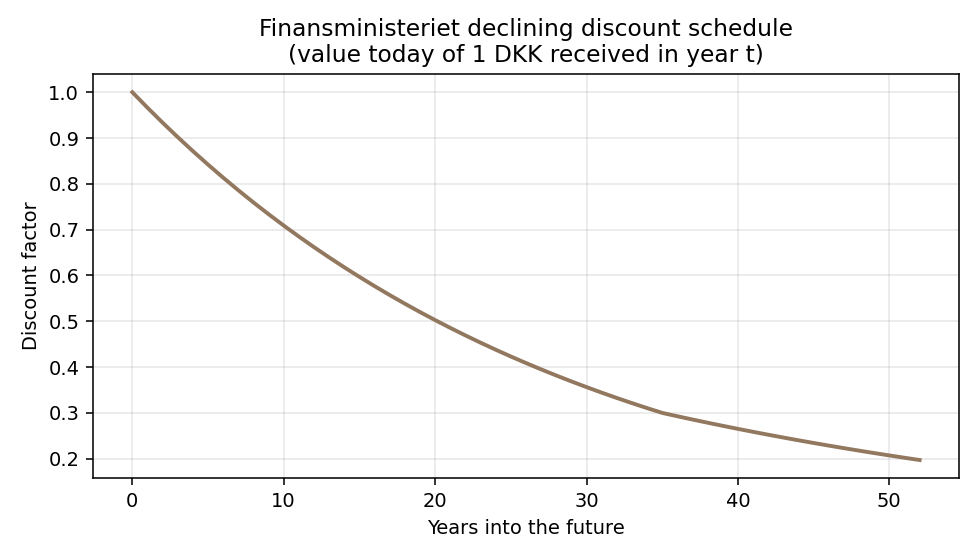
\includegraphics[width=0.62\linewidth]{discount_schedule.png}
\caption{Finansministeriet declining discount schedule: present value today of
one krone received in year $t$.}
\label{fig:discount}
\end{figure}

% ===========================================================================
\section{Evidence anchoring of the parameters}
% ===========================================================================
The transition and destination parameters are \emph{directional anchors} drawn
from named public sources, not exact register extractions for the 18--30
cohort. They should be replaced with precise figures before any external claim;
the point of the model is to make each assumption explicit and testable.

\begin{table}[H]
\centering
\caption{Literature/register-anchored default parameters.}
\label{tab:params}
\small
\begin{tabular}{@{}llp{7.4cm}@{}}
\toprule
Parameter & Default & Anchor \\
\midrule
\texttt{share\_permanent} & 0.55 & (S1) Post-2013 young FP grants mostly permanent; revocations rare \\
$q_{\text{fp}}$ control / treated & 0.015 / 0.030 & (S1, S3) Revocation rare; initiative $\approx$ doubles it \\
dest.\ split (emp/fleks/other) & 0.20 / 0.45 / 0.35 & (S2) fleksjob dominates, ordinary jobs a minority \\
$q_{\text{res,work}}$ control / treated & 0.10 / 0.15 & (S2, S3) $\sim\tfrac14$ of completed forl\o b reach work/fleksjob \\
$q_{\text{res,fp}}$ control / treated & 0.10 / 0.075 & (S2) $\sim\tfrac13$ progress to FP; initiative prevents some \\
\bottomrule
\end{tabular}
\end{table}

\noindent\textbf{Sources.}
\begin{description}[nosep,leftmargin=2.6em,style=nextline]
  \item[(S1)] Reform of f\o rtidspension and fleksjob (Lov nr.\ 1380 af
    23/12/2012, in force 1 Jan 2013) and DST/STAR statistics on revocations
    (frakendelser).
  \item[(S2)] STAR / jobindsats.dk result statistics for completed
    ressourceforl\o b; Rigsrevisionen, \emph{Beretning om ressourceforl\o b}
    (9/2019).
  \item[(S3)] IPS (Individual Placement and Support) evidence --- international
    meta-analyses and Danish IPS trials --- employment effects of about
    $+10$ to $+15$ percentage points, used as an \emph{upper} anchor for the
    initiative's effect. A volunteer bridging model is lighter-touch than full
    IPS, so defaults sit in the lower part of that range.
\end{description}

% ===========================================================================
\section{Results}
% ===========================================================================
\subsection{Headline}
With the anchored defaults the model yields the figures in
Table~\ref{tab:headline}. The per-participant saving is modest and highly
skewed: most individuals never exit (so their saving is just the negative
programme cost), while a minority of successful exits carry large,
long-horizon savings. Crucially, the value is concentrated in the
ressourceforl\o b track, consistent with the intuition that preventing
\emph{progression into} permanent FP is worth far more than reversing an
already-granted FP.

\begin{table}[H]
\centering
\caption{Headline results, anchored defaults (synthetic cohort, $n=\num{1500}$).}
\label{tab:headline}
\small
\begin{tabular}{@{}lr@{}}
\toprule
Quantity & Value \\
\midrule
Mean NPV saving / participant & \dkk{32000} (approx.) \\
Median NPV saving / participant & \dkk{10000} (approx.) \\
Share of Monte-Carlo draws net-positive & $27\%$ \\
Mean saving --- f\o rtidspension track & \dkk{11000} (approx.) \\
Mean saving --- ressourceforl\o b track & \dkk{52000} (approx.) \\
\bottomrule
\end{tabular}
\end{table}

\begin{figure}[H]
\centering
\begin{subfigure}{0.58\linewidth}
  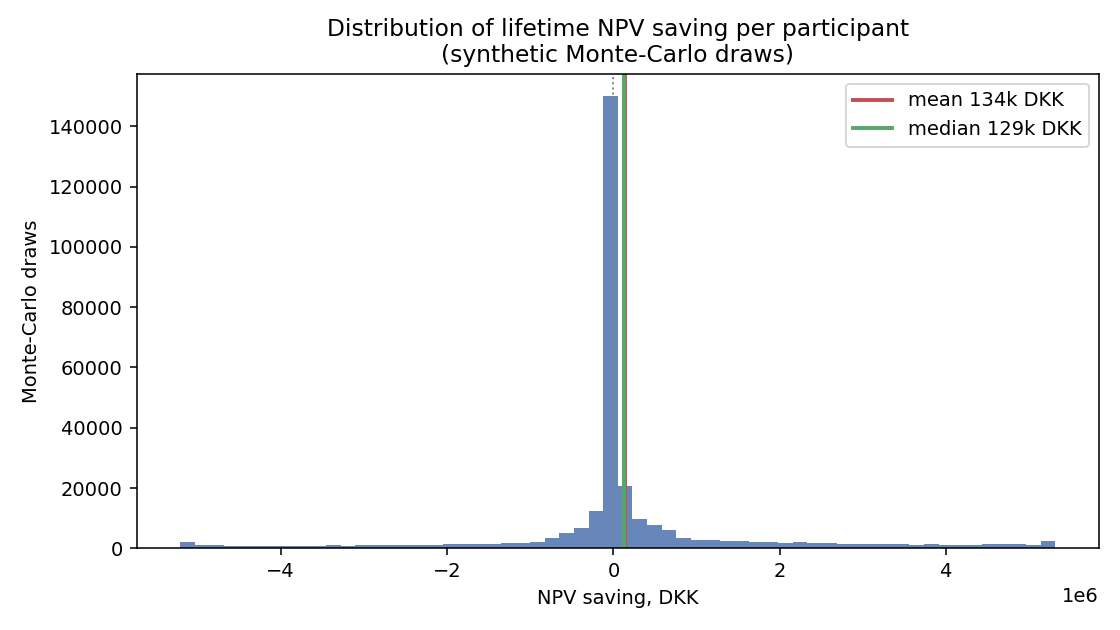
\includegraphics[width=\linewidth]{npv_distribution.png}
  \caption{Distribution of per-draw NPV savings.}
  \label{fig:dist}
\end{subfigure}\hfill
\begin{subfigure}{0.40\linewidth}
  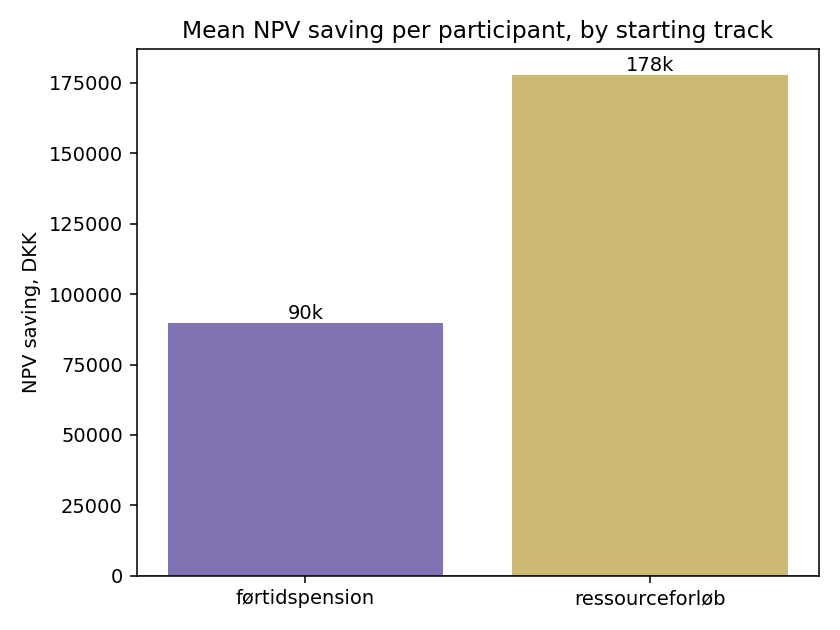
\includegraphics[width=\linewidth]{npv_by_track.png}
  \caption{Mean saving by starting track.}
  \label{fig:track}
\end{subfigure}
\caption{The saving is right-skewed (a) and concentrated in the
ressourceforl\o b track (b).}
\label{fig:headline}
\end{figure}

\subsection{One-way sensitivity (tornado)}
Varying one assumption at a time (Figure~\ref{fig:tornado}) shows the result is
most sensitive to the FP exit treatment effect $\Delta q$ and the discount
rate, then the RES$\to$work effect and the permanent share. This ranking is
more defensible than the headline level itself.

\begin{figure}[H]
\centering
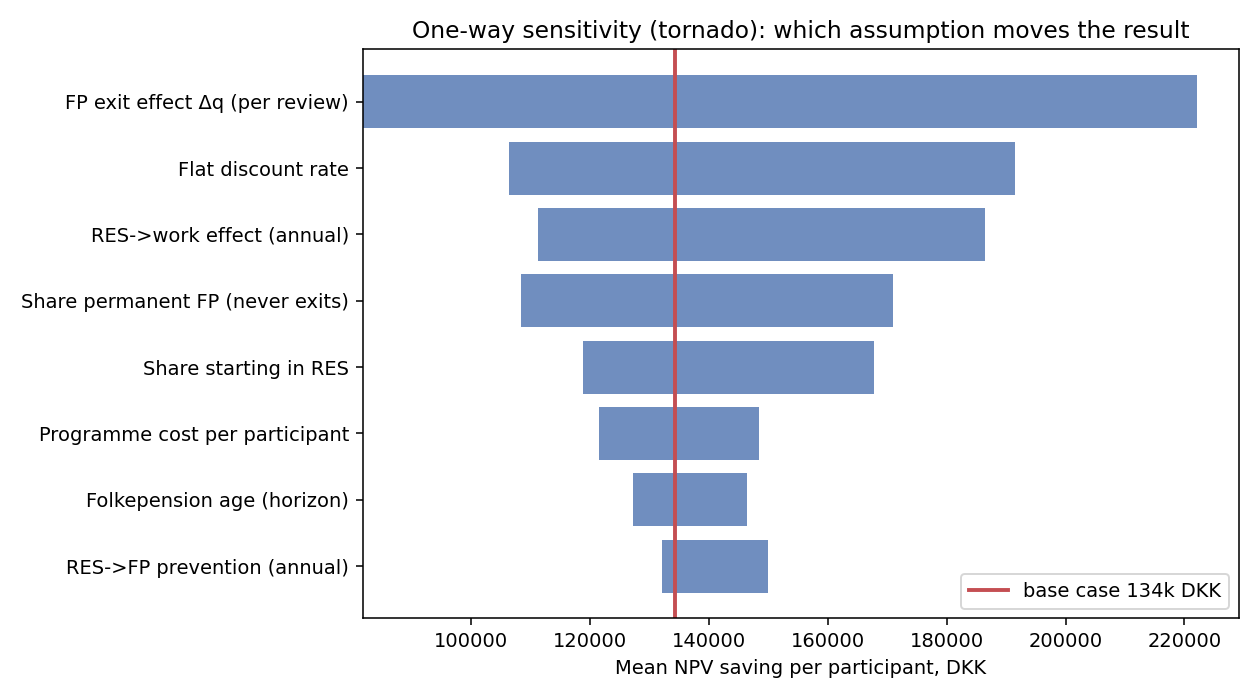
\includegraphics[width=0.85\linewidth]{tornado_sensitivity.png}
\caption{One-way sensitivity. Bars span the low/high value of the mean saving
as each driver is varied alone; the red line is the base case.}
\label{fig:tornado}
\end{figure}

\subsection{Probabilistic sensitivity analysis}
The PSA (\texttt{probabilistic\_sensitivity.py}) samples \emph{all} uncertain
parameters jointly --- Beta distributions for probabilities, a Dirichlet for the
destination split, Normal for costs, and Uniform for the treatment uplifts and
discount rate --- and reruns the simulation \num{800} times. The resulting
uncertainty fan (Figure~\ref{fig:fan}) and driver ranking
(Figure~\ref{fig:prcc}) give the report's most honest summary:

\begin{itemize}[nosep]
  \item mean of the mean-saving $\approx$ \dkk{37000};
  \item $95\%$ credible interval $\approx [\,-\dkk{6000};\ \dkk{117000}\,]$;
  \item $P(\text{saving} > 0) \approx 94\%$.
\end{itemize}

So even under joint uncertainty the initiative is very likely to save money,
but the \emph{size} of the saving is governed mainly by the
fleksjob-versus-ordinary-employment destination mix
(\texttt{p\_employment}, \texttt{net\_cost\_fleksjob}) and the relapse rate ---
not by the treatment effect alone. That is where better Danish register data
would most improve the estimate.

\begin{figure}[H]
\centering
\begin{subfigure}{0.49\linewidth}
  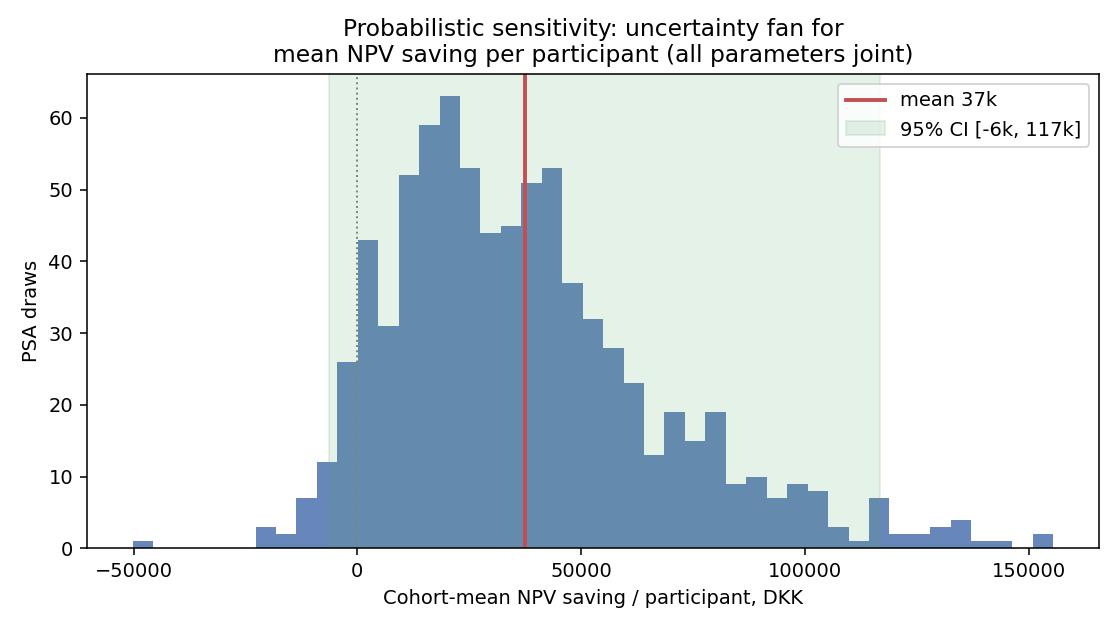
\includegraphics[width=\linewidth]{psa_fan.png}
  \caption{Uncertainty fan for the mean saving.}
  \label{fig:fan}
\end{subfigure}\hfill
\begin{subfigure}{0.49\linewidth}
  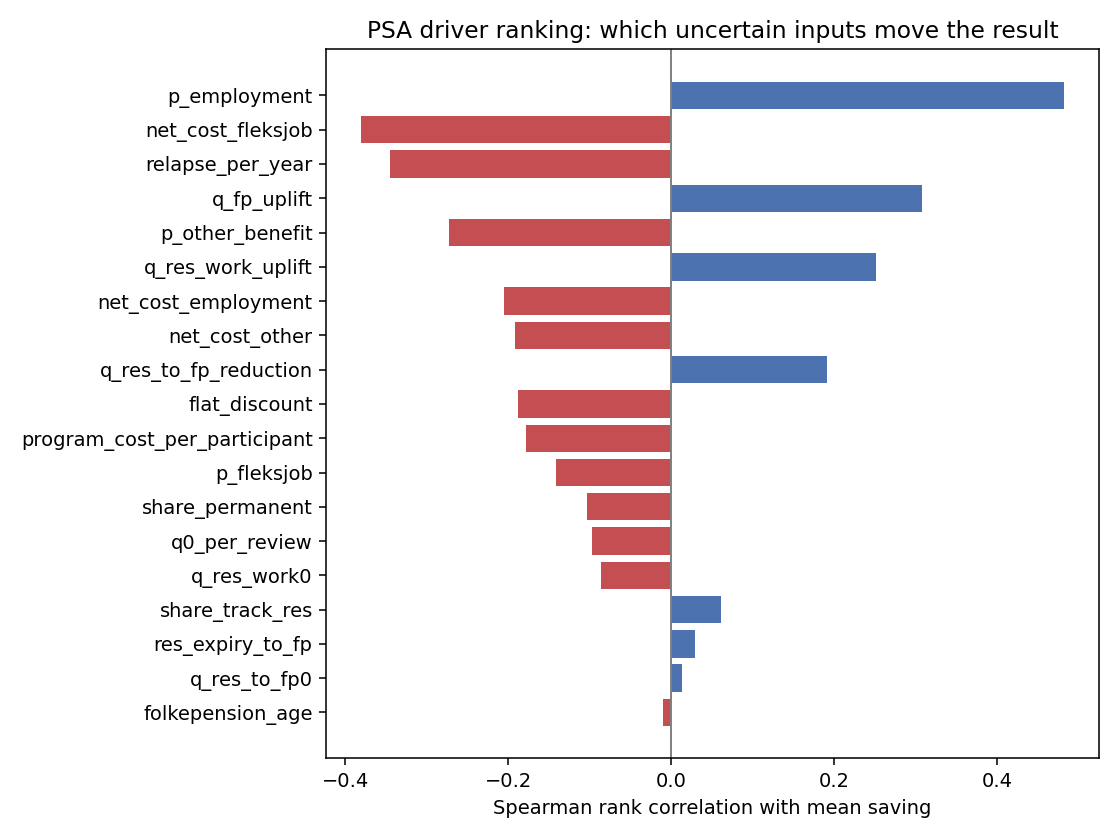
\includegraphics[width=\linewidth]{psa_prcc.png}
  \caption{Driver ranking (rank correlation).}
  \label{fig:prcc}
\end{subfigure}
\caption{Probabilistic sensitivity analysis: the full joint-uncertainty fan
(a) and which inputs move the result (b).}
\label{fig:psa}
\end{figure}

% ===========================================================================
\section{Limitations}
% ===========================================================================
\begin{enumerate}[nosep]
  \item \textbf{Synthetic data.} Levels are illustrative; the anchored
    parameters are directional, not exact register extractions for the 18--30
    cohort.
  \item \textbf{No causal identification.} The treatment effect $\Delta q$ is an
    input anchored to IPS evidence, not an estimate for \emph{this} programme.
    A credible own estimate would need an RCT or quasi-experiment.
  \item \textbf{Selection.} Participants of a voluntary programme differ from
    non-participants; a naive $\Delta q$ overstates savings.
  \item \textbf{Partial fiscal scope.} We count benefits and income tax only ---
    not health-care use, VAT, or quality-of-life gains, which would
    \emph{raise} the social value.
  \item \textbf{Horizon risk.} Folkepension age and the discount schedule are
    indexed and uncertain; both are stress-tested in the tornado and the PSA.
\end{enumerate}

% ===========================================================================
\section{Reproducibility}
% ===========================================================================
All randomness is controlled by a fixed seed. The full pipeline is:
\begin{verbatim}
python early_retirement_savings_model.py   # headline + tornado table
python export_synthetic_register.py        # data/synthetic_cohort.csv + codebook
python make_figures.py                     # figures/*.png
python probabilistic_sensitivity.py        # PSA fan, driver ranking, psa_draws.csv
\end{verbatim}

\paragraph{Conclusion.}
Framed as a present-value calculation in the same spirit as the mink
compensation, a low-cost bridging initiative for young disability-benefit
recipients is very likely to be fiscally self-financing, with the bulk of the
value coming from \emph{preventing progression into permanent f\o rtidspension}
via the ressourceforl\o b track. The size of the prize, however, hinges on
where successful participants land --- a question only Danish register data can
settle.

\end{document}
